\documentclass[a4paper,12pt]{report}
\newcommand{\HRule}{\rule{\linewidth}{0.5mm}}
\addtolength{\oddsidemargin}{-1.cm}
\addtolength{\textheight}{3.5cm}
\addtolength{\textwidth}{2cm}
\addtolength{\topmargin}{-2cm}


\usepackage[pdftex]{graphicx}
\usepackage[utf8]{inputenc}
\usepackage[english]{babel}



%define the tile

\title{Phase 1 Mini Project}
\begin{document}

\setlength{\parskip}{6pt}


%generate title

\begin{titlepage}
\begin{center}

% top section of title page


\includegraphics[width=1\textwidth]{./up-logo.jpg}\\[0.4cm]  
\textsc{\LARGE COS 301}\\[1.5cm]
\textsc{\LARGE Department Of Computer Science}\\[0.3cm]

%Title

\HRule \\[0.4cm]
{ \huge \bfseries Phase 1 Mini Project}\\[0.1cm]
\HRule \\[0.4cm]

% Group Members 

\begin{minipage}{0.4\textwidth}
\begin{flushleft} \large

\emph{Group Members:}\\
\emph{}\\
TJR \textsc{Kirker}
\emph{}\\
\emph{}\\
KK \textsc{Kgwete}
\emph{}\\
\emph{}\\
JD \textsc{Marx}
\emph{}\\
\emph{}\\
LL \textsc{Molokomme}
\emph{}\\
\emph{}\\
P \textsc{Mtsweni}
\emph{}\\
\emph{}\\
X \textsc{Ntshingila}
\emph{}\\
\emph{}\\
T \textsc{Ntsaba}
\emph{}\\
\emph{}\\
D \textsc{Obo}

\end{flushleft}
\end{minipage}
\begin{minipage}{0.4\textwidth}
\begin{flushright} \large

\emph{Student numbers:} \\
\emph{}\\
u11152402
\emph{}\\
\emph{}\\
u11247143
\emph{}\\
\emph{}\\
u12105202
\emph{}\\
\emph{}\\
u11197961
\emph{}\\
\emph{}\\
u11116774
\emph{}\\
\emph{}\\
u13410378
\emph{}\\
\emph{}\\
u10668544
\emph{}\\
\emph{}\\
u13134885


\end{flushright}
\end{minipage}
\vfill

% bottom section of title page

{\large \today}
\end{center}
\end{titlepage}
\setcounter{chapter}{1}
\renewcommand{\thesection}{\arabic{section}}

\section{System Overview}
\texttt{The BuzzSystem aims to enhance the learning process by providing a platform in which Lecturers, Tutors and Students can discuss concepts covered in class in a more user friendly manner which is appealing to students; consequently this will deepen their understanding of the concepts and improve their overall performance. 
\emph{}\\
This is achieved by introducing social networking elements such as tagging and gaming abilities such as earning points, because of these introductions  the system will not only encourage competitiveness but also provide reporting functionalities which will indicate the performance of individual users and the system as a whole. 
}

\newpage
\section{Functional requirements and application design}

\subsection{Use case prioritization}

\textbf{Critical}
\begin{itemize}
	\item UserManagement
	\item Posting
	\item BuzzSpace
\end{itemize}

\textbf{Important}
\begin{itemize}
	\item Category
	\item Vote
	\item Important
\end{itemize}

\textbf{Nice to Have}
\begin{itemize}
	\item tagging
	\item Rewarding
\end{itemize}

\subsection{Use case/Services contracts}
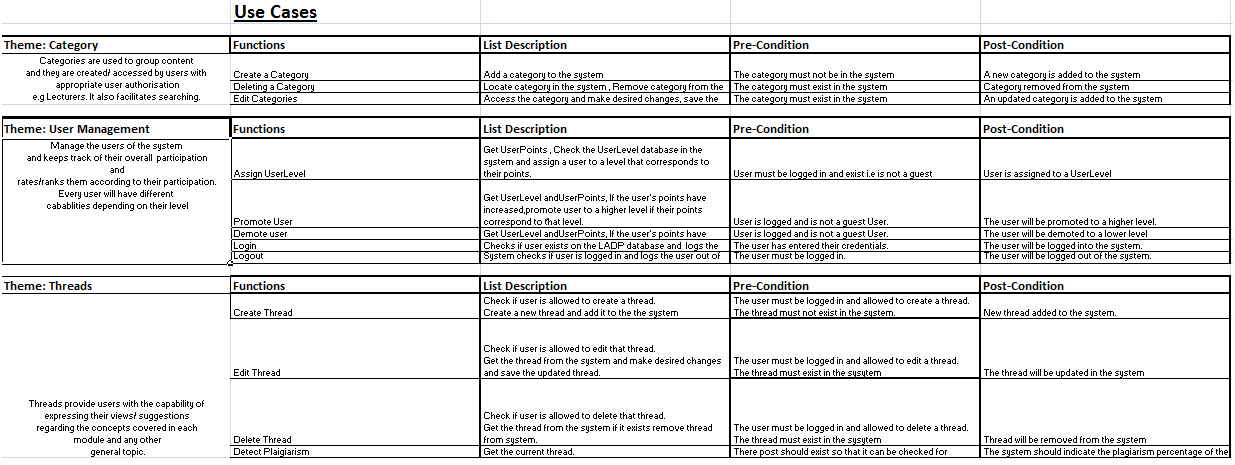
\includegraphics[width=1\textwidth]{./Use_case_A.png}\\[0.4cm]
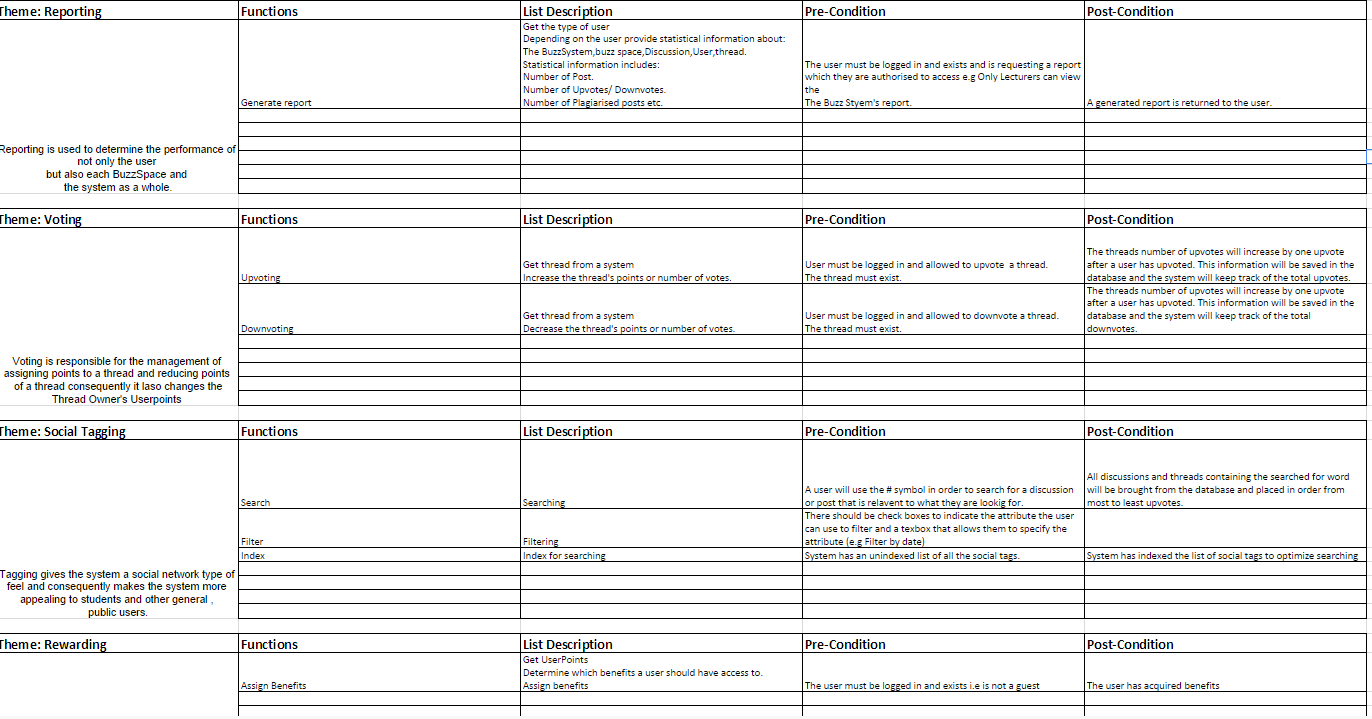
\includegraphics[width=1\textwidth]{./Use_case_B.png}\\[0.4cm] 
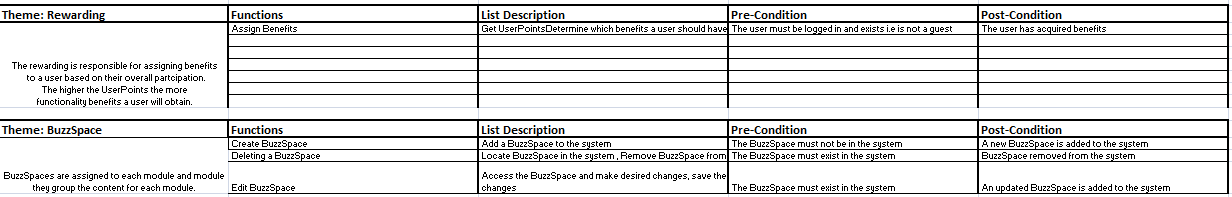
\includegraphics[width=1\textwidth]{./Use_case_C.png}\\[0.4cm]

\newpage
\subsection{Required functionality}
\textsc{Social Tag}
\emph{}\\
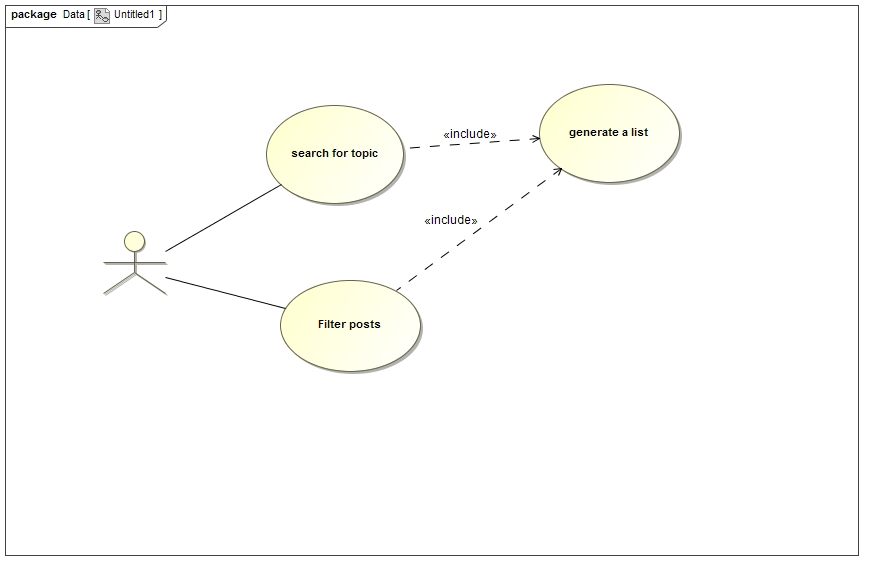
\includegraphics[width=1\textwidth]{./socialtag.jpg}\\[0.4cm]

\textsc{Rewarding}
\emph{}\\
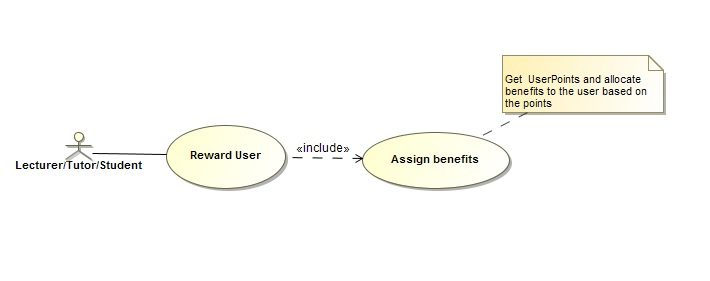
\includegraphics[width=1\textwidth]{./Use_Case_Diagram_RewardUser.jpg}\\[0.4cm] 

\newpage
\textsc{UserManagement}
\emph{}\\
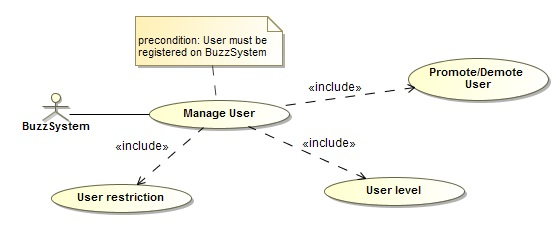
\includegraphics[width=1\textwidth]{./Activity_Diagram_UserManagement.jpg}\\[0.4cm]


\textsc{Vote}
\emph{}\\
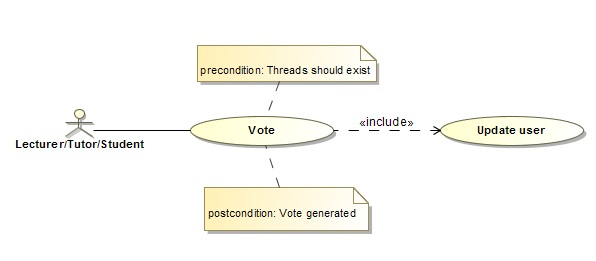
\includegraphics[width=1\textwidth]{./Use_Case_Diagram_Vote.jpg}\\[0.4cm]

\newpage
\textsc{threads}
\emph{}\\
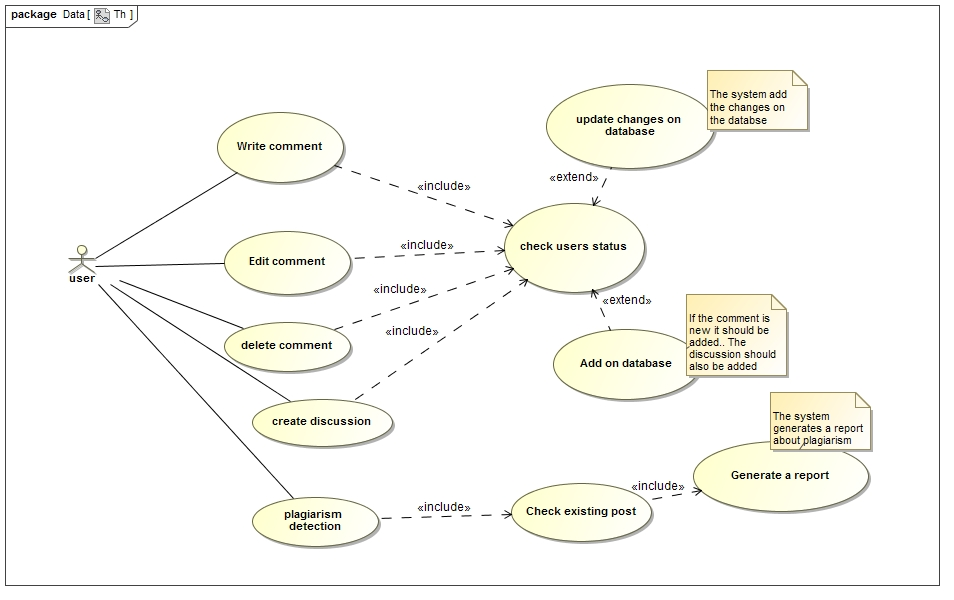
\includegraphics[width=1\textwidth]{./uthreads.jpg}\\[0.4cm]  

\textsc{Reporing}
\emph{}\\
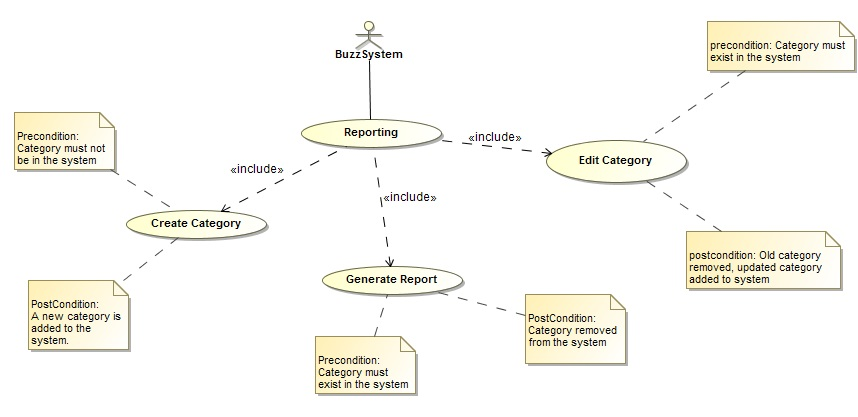
\includegraphics[width=1\textwidth]{./Activity_Diagram_CreateCategory.jpg}\\[0.4cm]


\newpage
\subsection{Process specifications}
 
\textsc{Login}
\emph{}\\
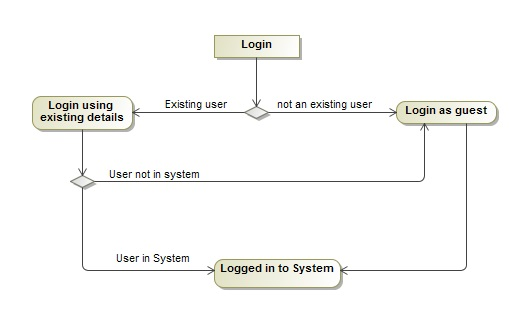
\includegraphics[width=1\textwidth]{./Activity_Diagram_Login.jpg}\\[0.4cm]  

\textsc{Rewarding}
\emph{}\\
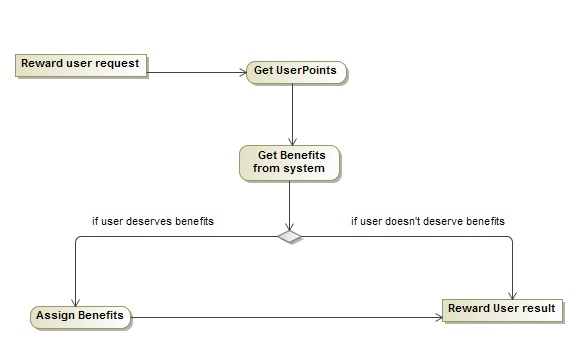
\includegraphics[width=1\textwidth]{./Activity_Diagram_RewardSystem.jpg}\\[0.4cm]
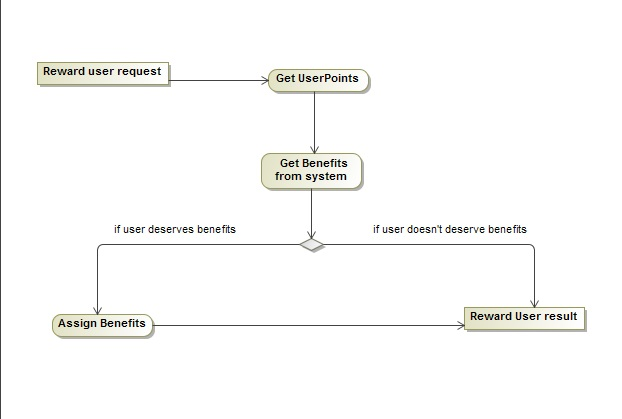
\includegraphics[width=1\textwidth]{./Activity_Diagram_RewardUser.jpg}\\[0.4cm] 

\newpage
\textsc{UserManagement}
\emph{}\\
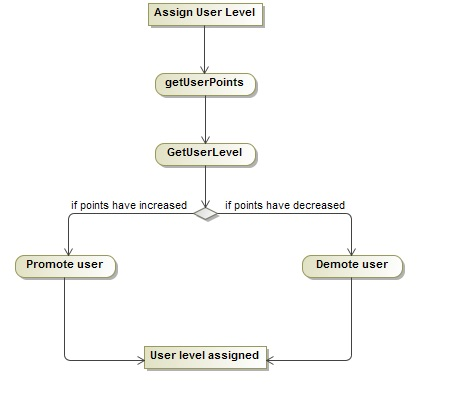
\includegraphics[width=1\textwidth]{./Use_Case_Diagram_UserManagement.jpg}\\[0.4cm] 

\newpage
\textsc{UserLevel}
\emph{}\\
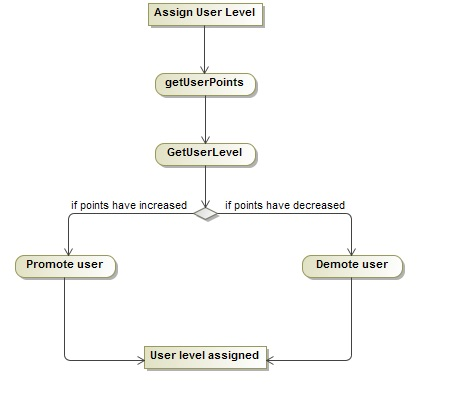
\includegraphics[width=1\textwidth]{./Activity_Diagram_UserLevel.jpg}\\[0.4cm]

\newpage
\subsection{Domain Model}
\emph{}\\
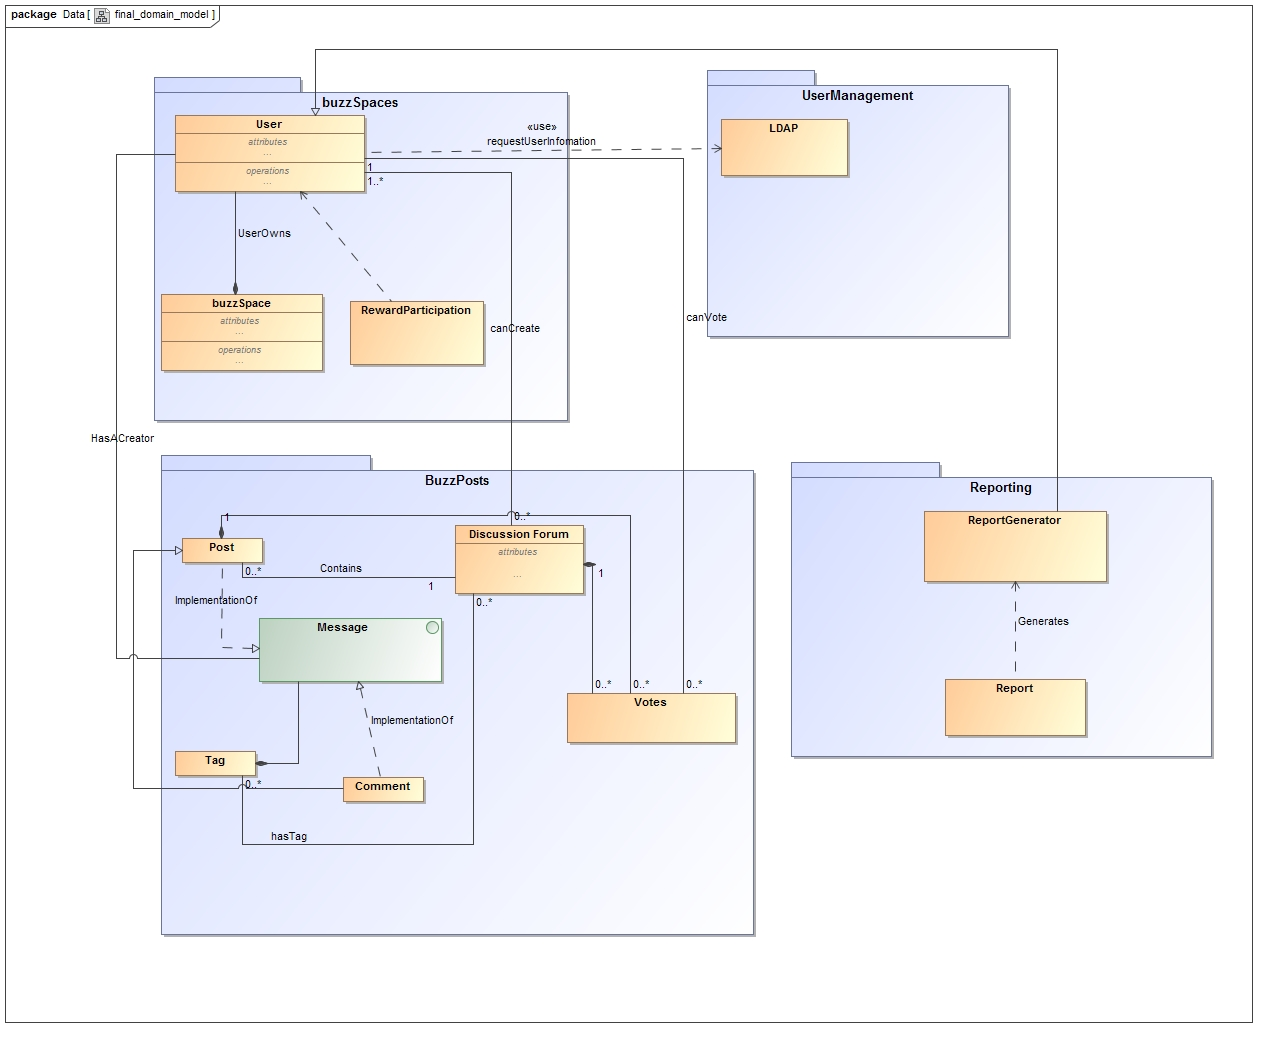
\includegraphics[width=1\textwidth]{./final_domain_model_a.jpg}\\[0.4cm]


\end{document}







